% !TEX root = ../risk_vs.tex
\section{Research vs Data Mining}\label{sec:pubvs}

We compare in detail the post-sample returns of peer-reviewed research to data mining. 

\subsection{Peer-Reviewed Predictor Data} \label{sec:pubvs-data-pub}
% see DataCounts.md

Peer-reviewed predictors come from the October 2024 release of the \citet{ChenZimmermann2021}  (CZ) dataset.  This dataset is built from 212 firm-level variables that were shown to predict returns cross-sectionally in academic journals. It covers the vast majority of firm-level predictors that can be created from widely-available data and were published before 2016. The CZ data is a uniquely accurate representation of the literature: unlike other large-scale replications, CZ show that their t-stats are generally a good match for the t-stats in the original papers.

CZ select their predictors to provide comprehensive coverage of predictors examined in previous  meta-studies (\citealt{mclean2016does}; \citealt{harvey2016and}; \citealt{green2017characteristics}; \citealt{Hou2020Replicating}). These meta-studies, in turn, aim for comprehensive coverage of academic cross-sectional stock return predictors. 

We drop five predictors that have fewer than 9 years of post-sample returns.  These predictors use specialized data sources that have been discontinued (e.g., the \citet{gompers2003corporate} governance index). This restriction makes our charts easier to interpret.

We drop an additional 29 predictors to ensure each paper is represented by at most 2 predictors. For papers that present more than 2 predictors, we only include the two predictors with the largest in-sample t-statistics. This filter ensures our results are representative of the literature, and do not over-weight papers that present numerous implementations of the same theme (e.g., \citepos{heston2008seasonality} seasonal momentum).\footnote{Previous versions of our study without this filter show very similar results.}

\subsection{Post-Sample Performance: Research vs Data Mining}\label{sec:pubvs-results}

We can now answer the question posed on page \pageref{sec:intro}. Does peer-reviewed research help predict cross-sectional returns compared to data mining?  

In our first test, we measure performance using the mean long-short return of strategies formed following the ``original paper'' specifications from CZ. These specifications match the original papers' predictability tests in terms of stock weighting and portfolio sorting (e.g., equal-weighted quintiles). We keep only predictors that produce mean long-short return t-stats $>$ 2.0 in the original samples. All strategies are signed to be positive and normalized to have 100 bps mean return in the original samples for ease of interpretation.

For each of these published strategies, we construct a data-mined benchmark by applying the same statistical treatment to the 29,000 accounting ratios. For each ratio, we construct t-stats based on the original papers' stock weighting and sample periods, filter for t-stats $>$ 2.0, sign and normalize to have $+100$ bps mean return in the original samples. Since finding t-stats $>$ 2.0 is rather common (Table \ref{tab:dm-oos}), on average, this process selects roughly 6,000 data-mined strategies for each published predictor. 

Figure \ref{fig:intro} compares the post-sample performance of the published strategies to their data-mined benchmarks. It plots trailing 5-year mean returns in event time, where the event is the end of the original sample periods.  

Post-sample, peer-reviewed (solid line) and data-mined (long-dash) predictors perform similarly. This similarity is seen both in the average post-sample performance, as well as in the event-time decay patterns. This result suggests that peer-reviewed research provides limited additional information about post-sample performance compared to data mining. 

Figure \ref{fig:pub-vs-dm-2} shows robustness to factor exposure. We calculate the abnormal return $r^{a}_{i,t}$ of strategy $i$ in month $t$:
\begin{align}
  r^{a}_{i,t} = r_{i,t}- \hat{\beta}_{i}^{(s)} f_t,
  \label{eq:abnormal_return}
\end{align}
where $r_{i,t}$ is the raw long-short return, $f_t$ is a vector of factor returns, and $\hat{\beta}_{i}^{(s)}$ is a row vector of betas estimated using sample $s$. The sample $s$ is either the original sample or the post-sample period. This separation ensures our t-stat filters do not produce look-ahead bias, but using full-sample betas leads to similar results (Internet Appendix \ref{sec:intapp-fullsamplerisk}). We then repeat the test in Figure \ref{fig:intro} using abnormal returns in place of the raw returns. This replacement is made throughout the analysis, implying that the t-stat $>$ 2.0 filters also use abnormal rather than raw returns.

\begin{figure}[!h]
  \caption{Factor Adjustments and Alternative Data Mining Methods}
  \label{fig:pub-vs-dm-2}
  Top panels repeat Figure \ref{fig:intro} using abnormal returns $r^{a}_{i,t} = r_{i,t}- \hat{\beta}_i^{(s)} f_t$, where $\hat{\beta}_i^{(s)}$ is estimated using sample-specific periods (in-sample or post-sample) and $f_t$ is the return of either the market less risk-free rate (CAPM) or the Fama-French three factors plus momentum (FF4). Bottom panels use alternative data mining methods: mining 3,000 ticker-based strategies (dashed line) or filtering for the top 5\% of t-stats (Panel (d)). Each predictor is normalized so that its mean original-sample return is 100 bps per month. Shaded area shows one standard error for the published predictors, clustered by calendar month and predictor. Figure \ref{fig:intro} is robust to factor adjustments. The statistical screen and number of strategies used for data-mining are unimportant but the type of data being mined is critical.

  \vspace{0.15in}
  
  \centering
  \subfloat[CAPM]{
  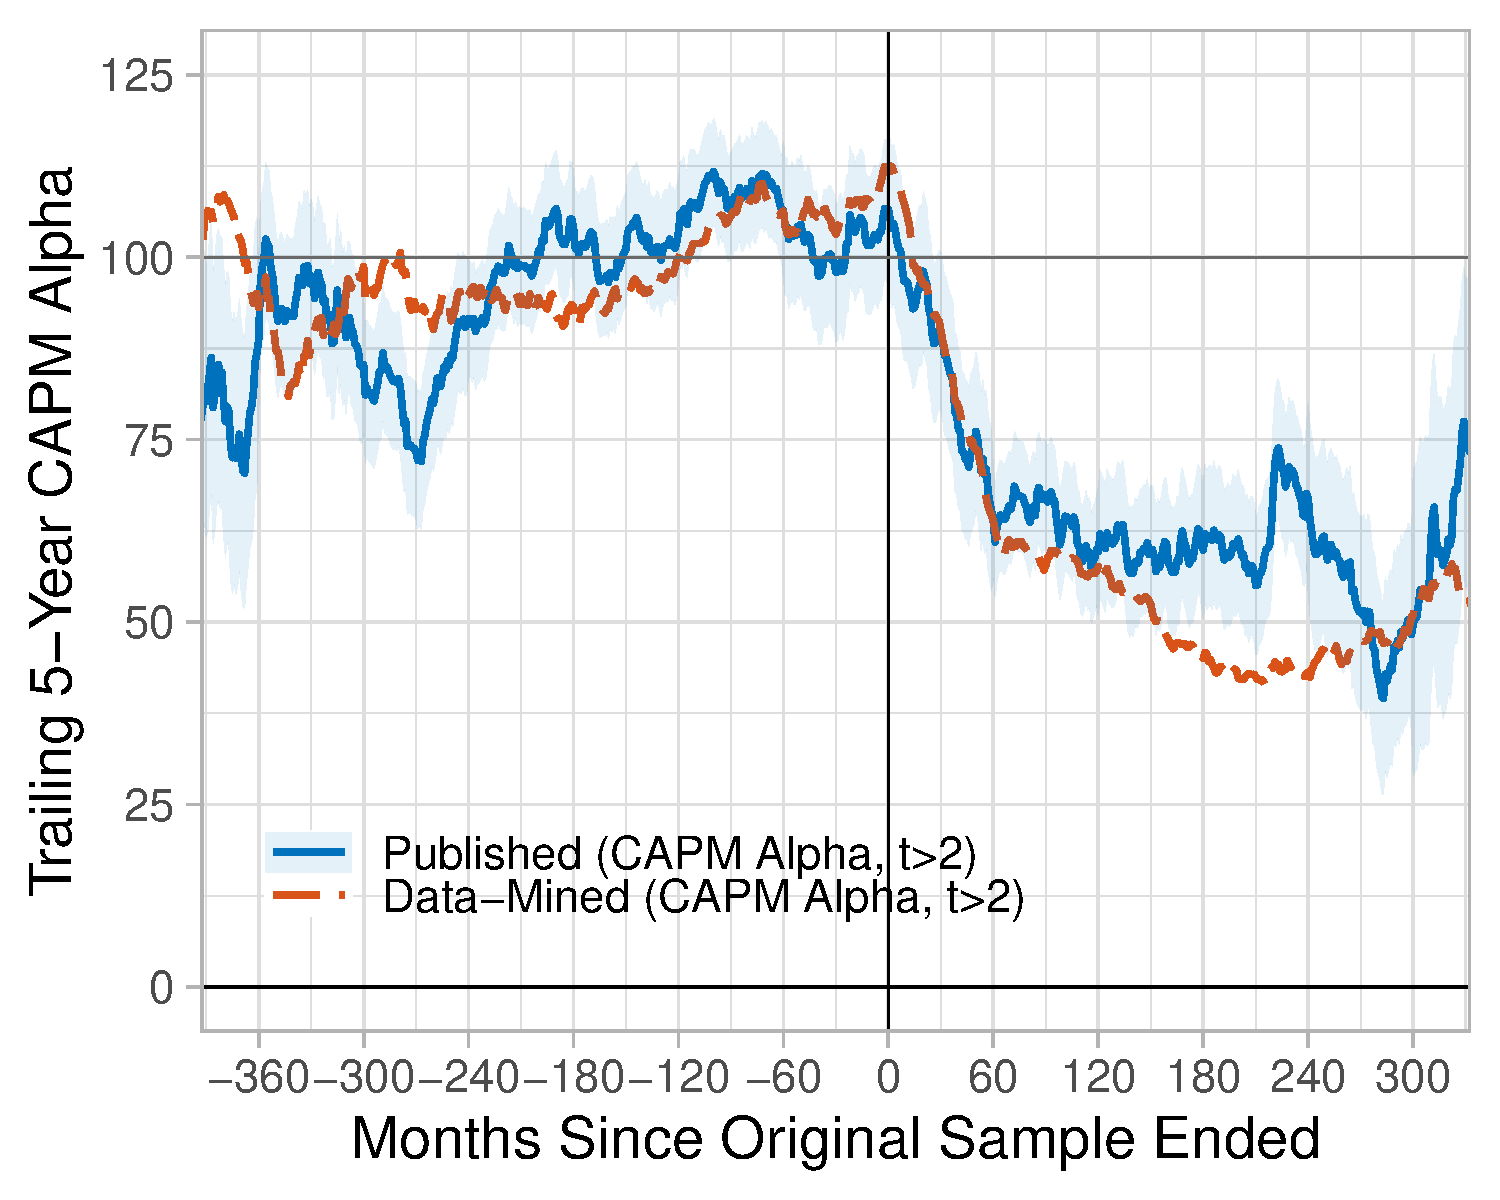
\includegraphics[width=0.48\textwidth]{exhibits/Fig_RiskAdj_capm_alpha_t2.pdf} 
  }
  \subfloat[FF3+Momentum]{
  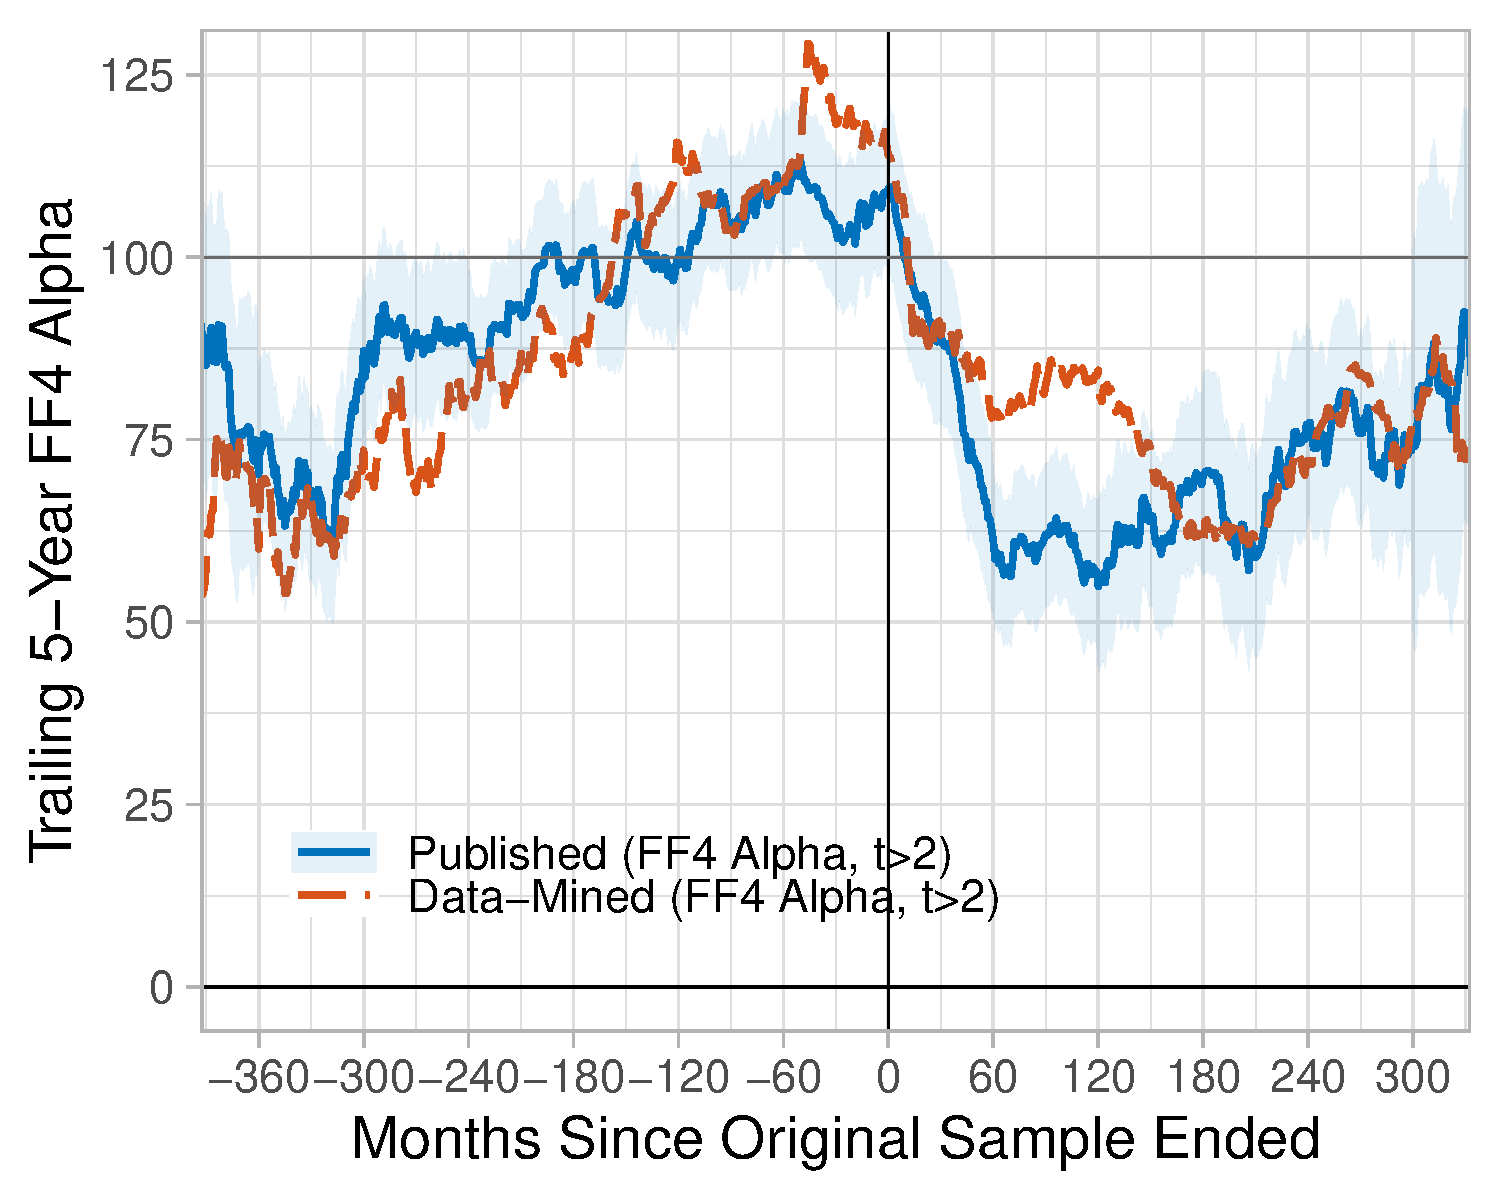
\includegraphics[width=0.48\textwidth]{exhibits/ff4/Fig_RiskAdj_ff4_alpha_t2.pdf}
  }\\
  \subfloat[Mining for t-stats $>$ 2.0 ]{
  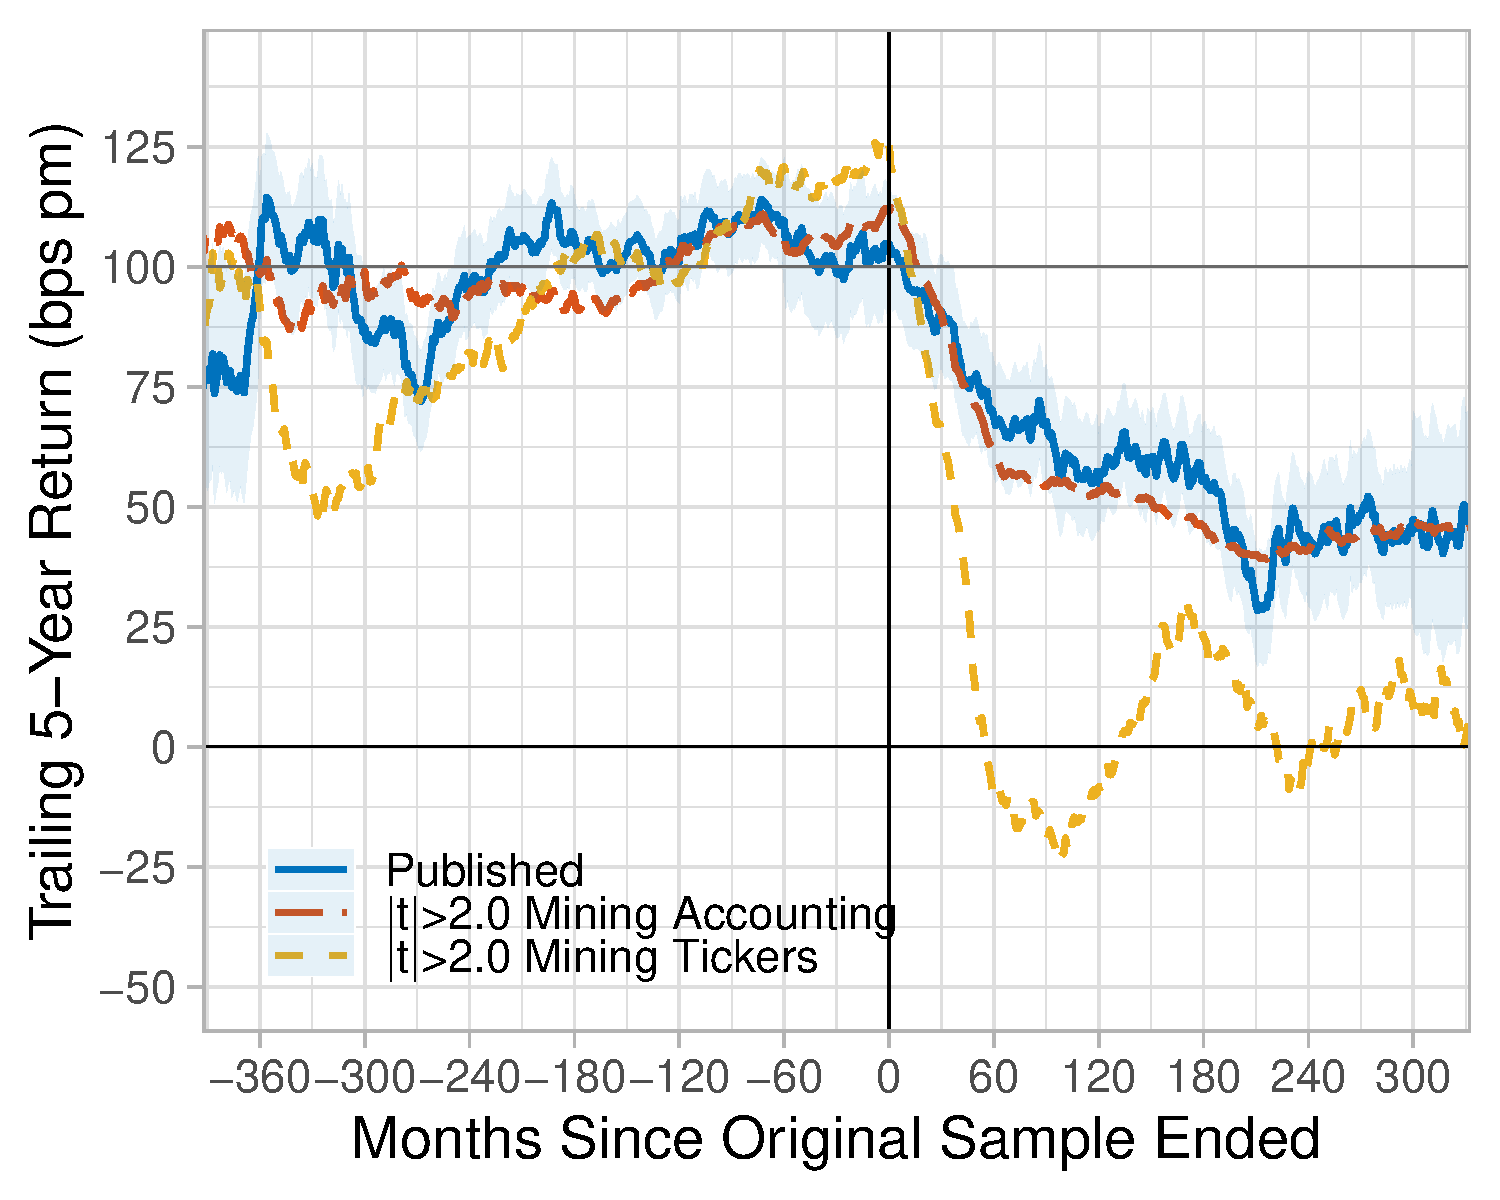
\includegraphics[width=0.48\textwidth]{exhibits/Fig_AltDM_SE_Calendar_t_min_2} 
  }
  \subfloat[Mining for top 5\% of t-stats]{
  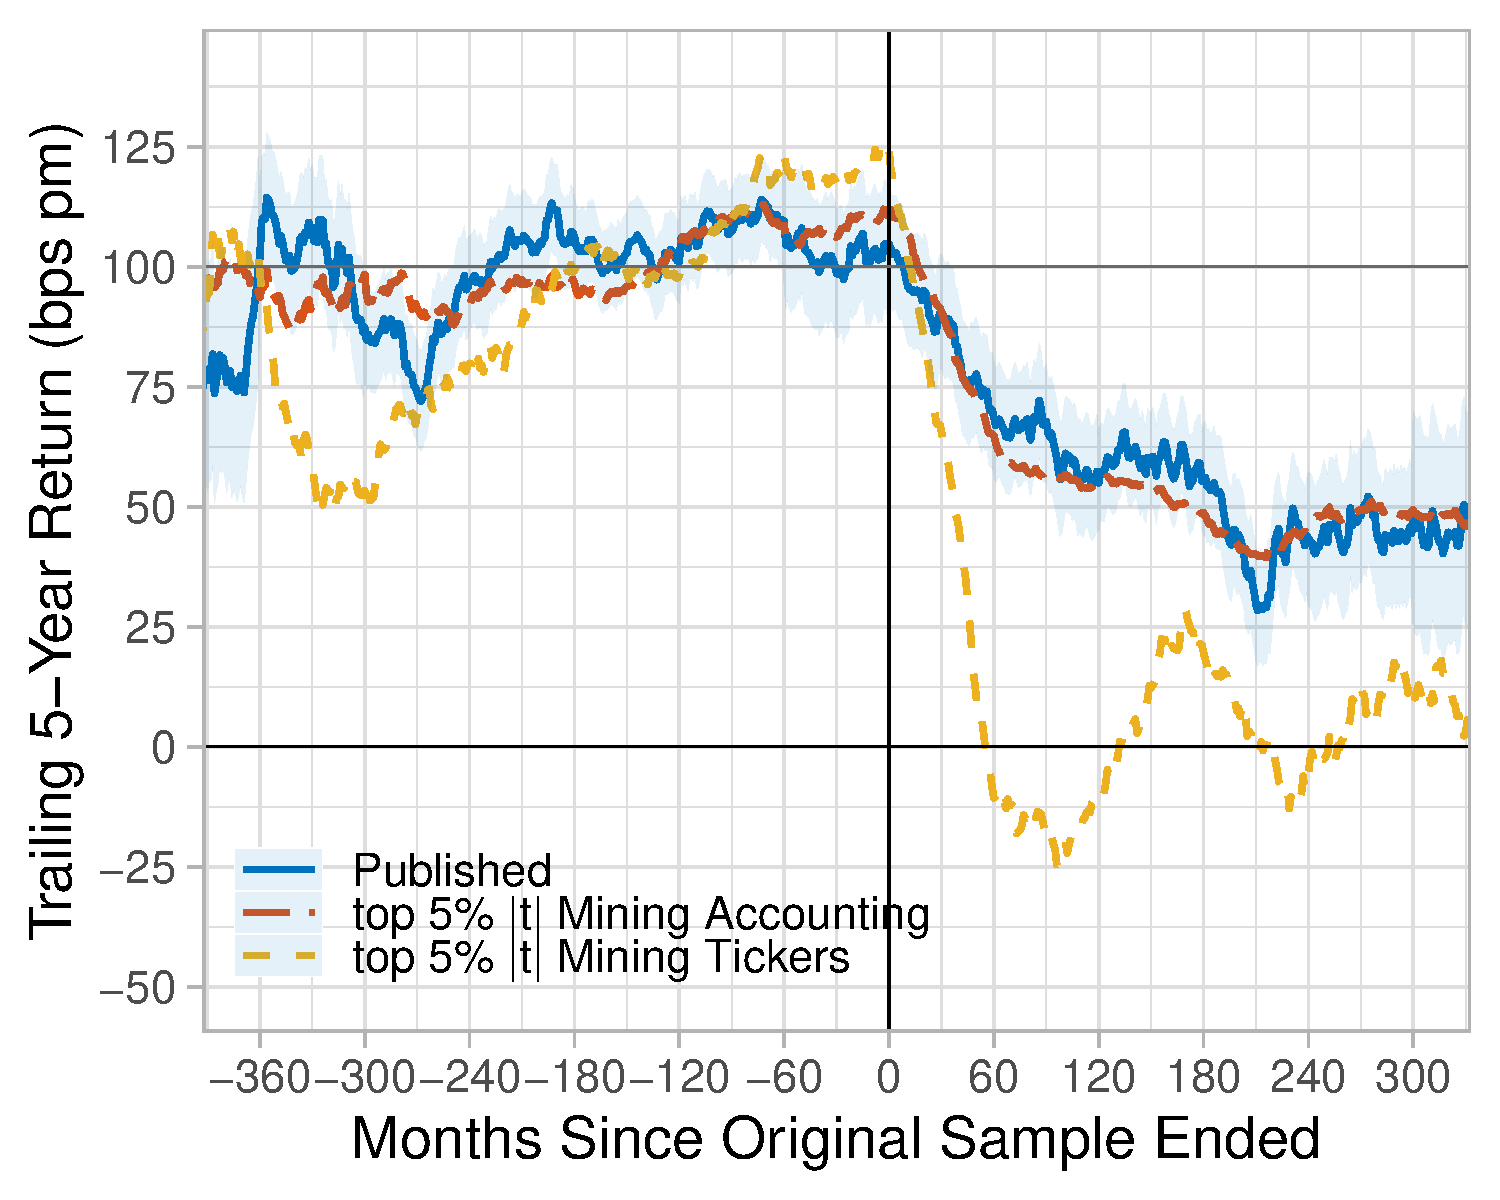
\includegraphics[width=0.48\textwidth]{exhibits/Fig_AltDM_SE_Calendar_t_rankpct_min_5}
  }
\end{figure}

Panel (a) of Figure \ref{fig:pub-vs-dm-2} shows that published predictors exhibit some outperformance relative to data-mined benchmarks in terms of CAPM-adjusted returns. However, the outperformance is modest. Post-sample, published predictors retain 60\% of their original-sample performance, compared to 52\% for data-mined benchmarks. Indeed, Panel (b) shows that if we measure abnormal returns relative to the Fama-French three factors + momentum, data mining slightly \emph{out}performs research. Overall, post-sample alphas are similar for published and data-mined predictors.

Further robustness is seen using many other controls. These include controls for research methods and quality (Sections \ref{sec:hetero} and \ref{sec:app-most-famous}), in-sample mean returns, in-sample t-statistics, and data sources (Appendix \ref{sec:app-robust}). We also find robustness to excluding data-mined predictors that are highly correlated with published predictors (Appendix \ref{sec:app-robust-manycor}).

\subsection{Alternative Data Mining Methods}\label{sec:pubvs-alt}

Our data mining process (Section \ref{sec:dm-data}) searches accounting ratios for t-stats $>$ 2.0. This method avoids look-ahead bias and is arguably the most straightforward way to mine data. However, one can think of alternative data mining methods, and use these to inspect the mechanism behind Figure \ref{fig:intro}. 

For example, one could use the data mining method proposed in \citet{harvey2017presidential}. Harvey asks his research assistant to ``form portfolios based on the first, second, and third letters of the ticker symbol,'' leading to 3,160 long-short portfolios. We interpret his instructions as follows:  Generate 26 portfolios by going long all stocks with a  first ticker letter of ``A,'' ``B,'' ``C,'' ..., and ``Z.''  Generate 26 portfolios by doing the same for the second ticker letter, and add a 27th portfolio for tickers that have no second ticker letter.  Apply the same to the third ticker.  This process results in $26 + 27 + 27 = 80$ long portfolios.  Finally, form $\binom{80}{2} = 3,160$ long-short portfolios by selecting all distinct pairs of the 80 long portfolios.  

The bottom panels of Figure \ref{fig:pub-vs-dm-2} compare published strategies to strategies based on ticker mining. Panel (c) applies the same predictability screen as in Figure \ref{fig:intro}: we screen for t-stats $>$ 2.0 in the original sample periods. Post-sample, the mean returns from mining tickers (short-dash line) are approximately zero. Thus, peer-reviewed research (solid line) is much more helpful for predicting returns than mining tickers. 

Panel (d) applies an alternative predictability screen: we screen for the top 5\% of t-stats in the original sample periods. Screening accounting ratios this way still leads to very similar returns to research. Screening tickers this way still leads to post-sample returns of around zero.

Figure \ref{fig:pub-vs-dm-2} illustrates two lessons about data mining. The first is that the data being mined is important. Accounting data are helpful for predicting returns, while ticker data are not. The second lesson is that mining more data does not necessarily mean worse out-of-sample performance. The accounting dataset is almost 10 times as large as the ticker dataset, yet it produces much stronger post-sample returns.  This result is consistent with false discovery controls, which typically depend on the distribution of test statistics rather than the number of tests (\citealt{benjamini1995controlling}; \citealt{chen2025t}).

% Summarize and interpret a bit
In summary, the average peer-reviewed publication leads to post-sample returns that are similar to those of a simple data mining process.

% ===============================================================
